\newpage
\section{Learning-based Character Animation}
将动作数据打入模型之中.
\subsection{Interactive Character Animation}

How to create interactive animation?
\begin{enumerate}
    \item check user input
    \item find a nice animation clip
    \item play it
\end{enumerate}


\subsubsection{Motion Graphs}

\begin{figure}[!htb]
    \centering
    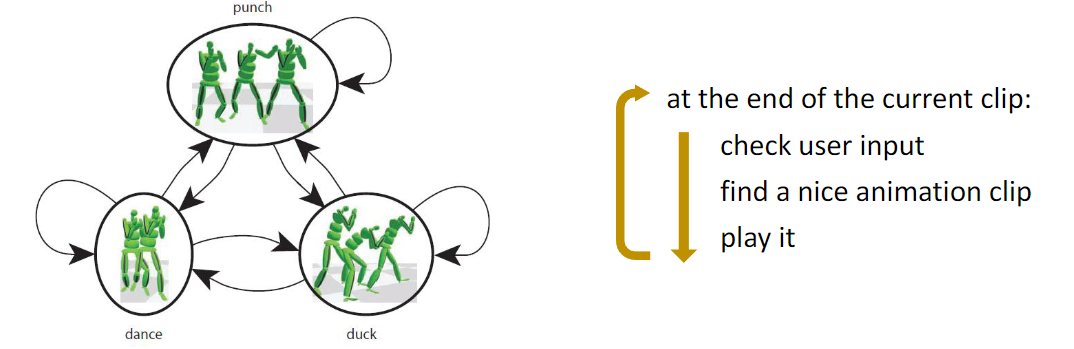
\includegraphics[width=0.88\linewidth]{pic/1056/Motion Graphs}
    \caption{Motion Graphs}
\end{figure}

靠自动的方法处理 clip 在质量上有很大的问题, 所以现在一般还是人工.


\subsubsection{Motion Fields}
如果需要提升响应速度, 则需要使用 Motion Fields / Motion Matching.

\begin{figure}[!htb]
    \centering
    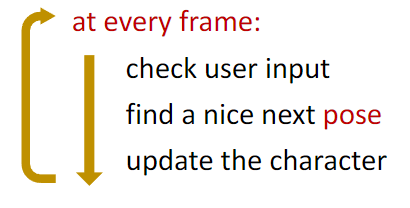
\includegraphics[width=0.42\linewidth]{pic/1056/Faster Response}
    \caption{Faster Response}
\end{figure}

\begin{figure}[!htb]
    \centering
    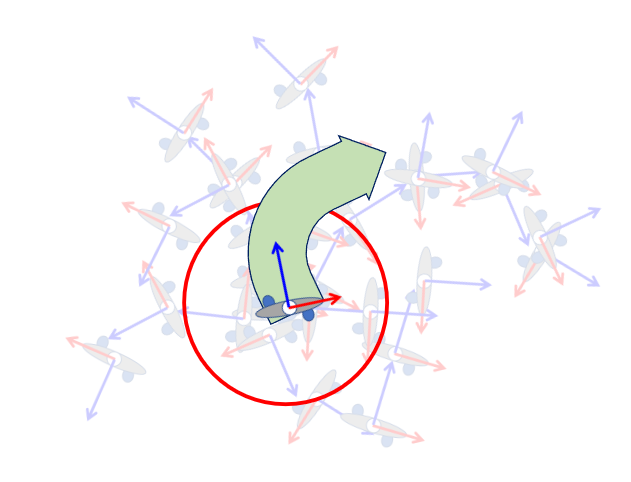
\includegraphics[width=0.618\linewidth]{pic/1056/Motion Fields}
    \caption{Motion Fields}
\end{figure}

对于某个状态, 可以找到一些最近邻姿态(红圈范围), 依据用户的输入, 赋予最近邻不同权重, 做个混合得到最后的姿态.

\begin{figure}[!htb]
    \centering
    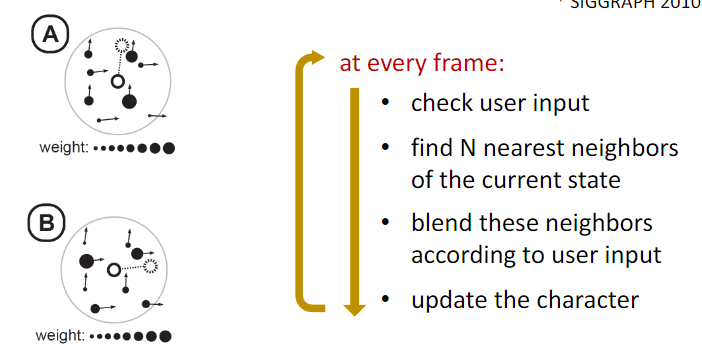
\includegraphics[width=0.88\linewidth]{pic/1056/Motion Fields2.png}
    \caption{Motion Fields}
\end{figure}

Motion Fields 响应快, 自由度比 Motion Graphs 高, 而且不需要做预处理, 不需要动作对齐. 

虽然 Motion Fields 效果很好, 但是没人用. 主要是因为 ``赋予最近邻不同权重'' 这一步不知道要怎么算. 论文里用了个 rl 处理这个权重, 而 rl 与方法强相关, 改一下可能就需要重新训练, 而且训练 rl 也不稳定. 

\subsubsection{Motion Matching}
启发自 Motion Fields, 简化了一些步骤, 加上了很好的工程实现, 得到了很好的效果. 

\begin{figure}[!htb]
    \centering
    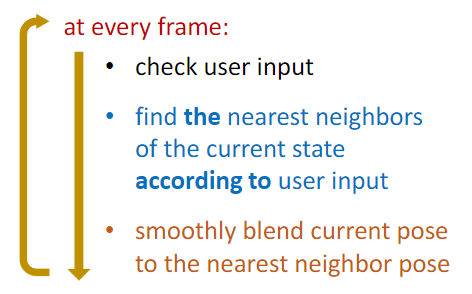
\includegraphics[width=0.618\linewidth]{pic/1056/Motion Matching}
    \caption{Motion Matching}
\end{figure}
主要是简化了寻找, 只寻找一个姿态, 这样就不需要做混合, 但是这个动作可能会有跳变, 所以会有个混合过度. 

Motion Matching 需要解决两个问题:
\begin{enumerate}
    \item We need a distance function / metric to define the nearest neighbor
    \begin{align*}
        \text{next\_pose} = \min_{i\in\text{Dataset}}\norm{x_{curr}-x_i}
    \end{align*}
    但这个函数效果不是很好, 可以选择混合特征获得更好的效果, $x$ 就是 feature vector. 
    \begin{figure}[!htb]
        \centering
        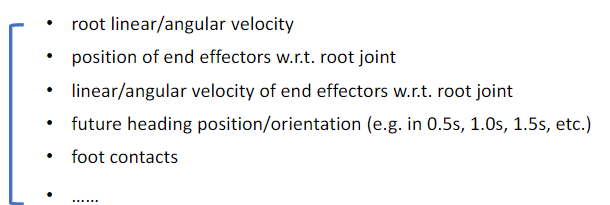
\includegraphics[width=0.618\linewidth]{pic/1056/A possible set of feature vectors}
        \caption{A possible set of feature vectors}
    \end{figure}
    
    \item We need a smooth motion
    \begin{itemize}
        \item 不是没帧都需要 matching, 只有用户输入时才进行
        \item Smoothly blend current pose to the target pose. 方法很多, 具体可以参考这个  \href{ https://www.theorangeduck.com/page/spring-roll-call}{blog}.
    \end{itemize}

    \item We need a good performance
    \begin{itemize}
        \item An efficient data structure for searching. e.g. KD-tree
        \item A efficient dataset. e.g. Dance card
    \end{itemize}
\end{enumerate}

缺陷: 不能解决滑步问题, 需要额外的 ik 处理之类的.

\subsection{Statistical Models of Human Motion}
希望产生数据集外自然的新的动作. 这里有个问题, 就是如何建模``自然''.

\subsubsection{The Low-dimensionality of Human Motions}
人的动作是有低维结构的数据. i.e. 比如对于关节旋转来说, 虽然有 22*3 = 66 个自由度, 但是绝大多数自由度是冗余的, 很多自由度是相互约束的. 以及更多的约束:
\begin{itemize}
    \item Coordinated arm/leg movement
    \item Musculoskeletal structure
    \item Laws of physics
\end{itemize}

具体来说, 人自然的动作是高维空间中的一个曲面. 
\begin{figure}[!htb]
    \centering
    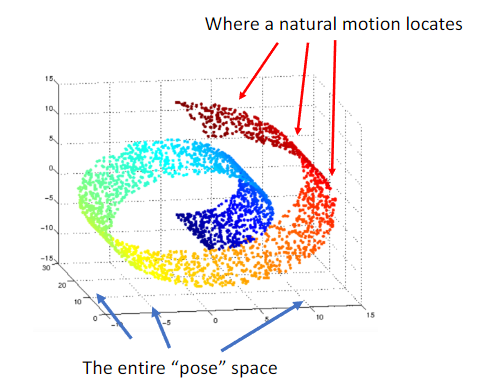
\includegraphics[width=0.618\linewidth]{pic/1056/The Low-dimensionality of Human Motions}
    \caption{The Low-dimensionality of Human Motions}
\end{figure}


\subsubsection{Principal Component Analysis (PCA)}
那么如何寻找这个自然的曲面呢? 一种方法是 PCA.

PCA 主要是寻找不同维度相对之间的关系, 以及可以据此作降维. 

\begin{figure}[!htb]
    \centering
    \begin{subfigure}{0.618\linewidth}
        \centering
        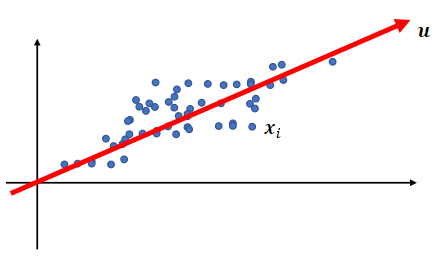
\includegraphics[width=\linewidth]{pic/1056/PCA}
        % \caption{}
    \end{subfigure}
    \begin{subfigure}{0.618\linewidth}
        \centering
        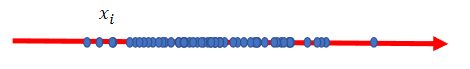
\includegraphics[width=\linewidth]{pic/1056/Projection }
        % \caption{}
    \end{subfigure}
    \caption{PCA}
\end{figure}


Projection of $\bx_i$ on $\bm u$: $w_i=\bx_i\cdot \bm u$, $w_i$ represents the coordinate of $\bx_i$ along the direction $\bm{u}$. We can approximate $\bx_i\approx w_i \bm u$. 
\begin{align*}
    \bx_i&= (\bx_i\cdot \bm u)\bm u + (\bx_i - (\bx_i\cdot \bm u)\bm u)\\
    &= w_i\bm u + (\bx_i - w_i\bm u)\\
    &\approx w_i\bm u 
\end{align*}

We need find a direction $\bm u$ such that $\norm{\bm u}=1$, and the projection of $\{ \bx_i \}$ on $\bm u$: $w_i=\bx_i\cdot \bm u$ have the maximal variance:
\begin{align*}
    \frac{1}{N}\sum_i(w_i-\bar{w})^2
\end{align*}

let
\begin{align*}
    X=\begin{bmatrix}
        (\bx_0-\bar{\bx}^\top)\\
        (\bx_1-\bar{\bx}^\top)\\
        \dots\\
        (\bx_N-\bar{\bx}^\top)\\
    \end{bmatrix}
\end{align*}
It can be proved that $\bm u$ is an eigenvector of $X^\top X$ corresponds to the largest eigenvalue. 

Note: now we can approximate $\bx_i\approx \bar{\bx}+w_i\bm u$.

Given a dataset $\{ \bx_i\}, \bx_i\in\R^N$, then PCA gives
\begin{align*}
    \bx_i=\bar{\bx}+\sum_{k=1}^nw_{i,k}\bm{ u}_k
\end{align*}
$\bm{u}_k$ is the $k$-th principal component. A direction in $\R^N$ along which the projection of $\{ \bx_i \}$ has the $k$-th maximal variance. $w_{i,k}=(\bx_i-\bar{\bx})\cdot \bm{u}_k$ is the score of $\bx_i$ on $\bm{u}_k$. 

The PCA can be computed by apply eigen decomposition on the covariance matrix
\begin{align*}
    \Sigma=X^\top X=U\begin{bmatrix}
        \sigma_1^2
    \end{bmatrix}U^\top
\end{align*}
$\sigma_i\ge \sigma_j\ge 0$ when $i<j$, corresponds to the Explained Variance. $U=[\bm{u}_1, \bm{u}_2,\dots,\bm{u}_N]$

e.g. PCA of walking. 

将一个 walking 的 motion 每一帧作为一个数据点, 做 PCA. 

\begin{figure}[!htb]
    \centering
    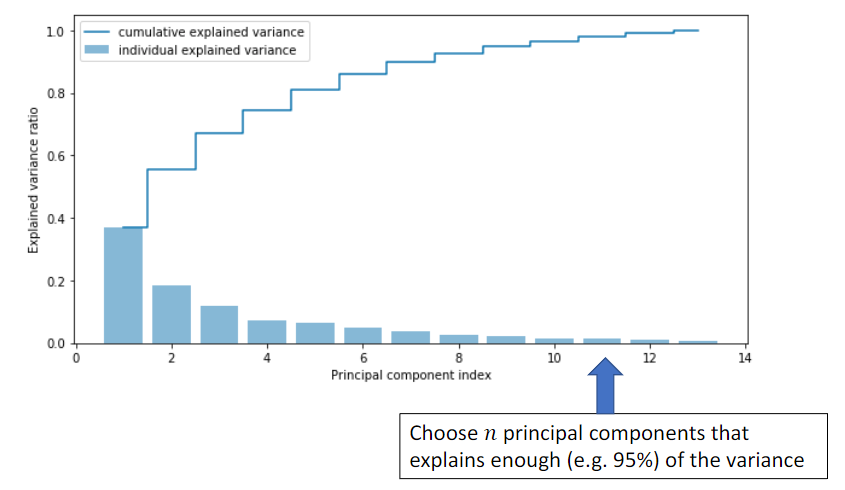
\includegraphics[width=0.618\linewidth]{pic/1056/PCA of walking}
    \caption{PCA of walking}
\end{figure}
cumulative explained variance 表示能恢复多少的原始动作. 

\begin{figure}[!htb]
    \centering
    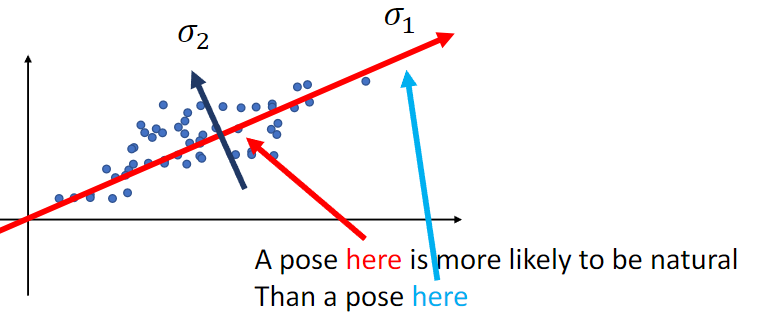
\includegraphics[width=0.618\linewidth]{pic/1056/natural}
    \caption{以 PCA 作为某种度量}
\end{figure}
A pose $\bx_i$ with smaller $\sum_k\left( \frac{w_{i,k}}{\sigma_k} \right)^2$ is more likely to be a good pose.



\paragraph{Character IK with a Reference Pose}在 Character IK 也可以用到这个度量, 作为先验. i.e.
\begin{align*}
    F(\theta)&=\frac{1}{2}\sum_i\norm{f_i(\btheta)-\tilde{\bx}_i}_2^2 + \frac{w}{2}\sum_k\left( \frac{(\btheta-\bar{\btheta})\cdot\bm{u}_k}{\sigma_k} \right)\\
    \btheta&=(\bm{t}_0, R_0, R_1, R_2, \dots)
\end{align*}

\subsubsection{Data Distribution}
为什么上面的可以判断动作是自然的? 因为我们假设动作是某种动力分布. 

$p(\bx)$: probability that $\bx$ is a natural pose. a set of data points $\{\bx_i\}\sim p(\bx)$.

Given a dataset of mocap poses $\{\bx_i\}$. How to find $p(\bx)$?

\begin{figure}[!htb]
    \centering
    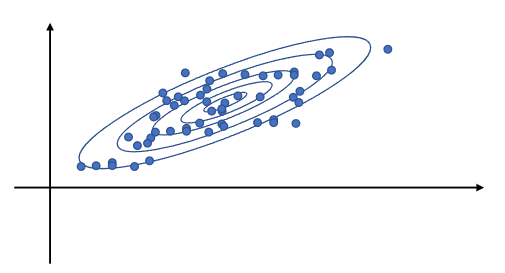
\includegraphics[width=0.618\linewidth]{pic/1056/Data Distribution}
    \caption{Data Distribution}
\end{figure}

\paragraph{Gaussian Distribution}直接假设其是个高斯分布, 然后直接根据公式计算. 

\paragraph{Character IK with a Motion Prior}基于上面那个 ik 公式, 可以变换为
\begin{align*}
    F(\theta)&=\frac{1}{2}\sum_i\norm{f_i(\btheta)-\tilde{\bx}_i}_2^2 -w\log p(\theta)\\
    \btheta&=(\bm{t}_0, R_0, R_1, R_2, \dots)
\end{align*}
所以上面那个 PCA 本质就是最小化概率密度函数负对数, 即最大化姿态出现的概率, 出现概率高的姿态一般是正常的. 

\paragraph{Motion Synthesis with a Motion Prior}Given a motion prior $p(\bx)$ learned from a set of data points $D=\{ \bx_i \}$ , Synthesize a motion $\bx$ that minimize the objective:
\begin{align*}
    F(x)=f(\bx)-w\log p(\bx)
\end{align*}
$x$ can represent a pose $\btheta$, or a motion clip, or any features of a motion.

但是一个高斯分布作为先验是不够的. 也有很多工作是扩展这个高斯模型, 比如用高斯混合模型(GMM), 高斯过程(GPLVM)等

但是超参数过多, 有很多很难的问题, 比如混合个数, 核函数等需要手动指定. 

现在就是用神经网络代替对运动先验的估计. 

\subsection{Learning-based Models}
\begin{figure}[!htb]
    \centering
    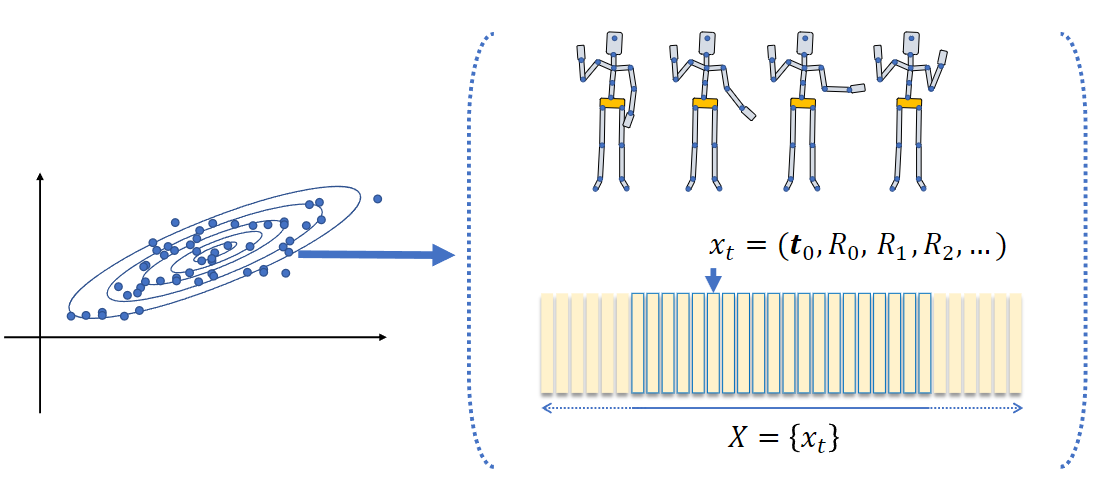
\includegraphics[width=0.618\linewidth]{pic/1056/Learning Motion Models}
    \caption{Learning Motion Models}
\end{figure}


Given a set of example motions $\{\bx_i\}\sim p(\bx)$, $p(\bx)$ is the probability that $\bx$ is a natural motion.

$p(X)=p(x_1,\dots,x_T)$ 表示一个 motion 的概率. 

\subsubsection{Learning Motion Models}

\begin{figure}[!htb]
    \centering
    \begin{subfigure}{0.88\linewidth}
        \centering
        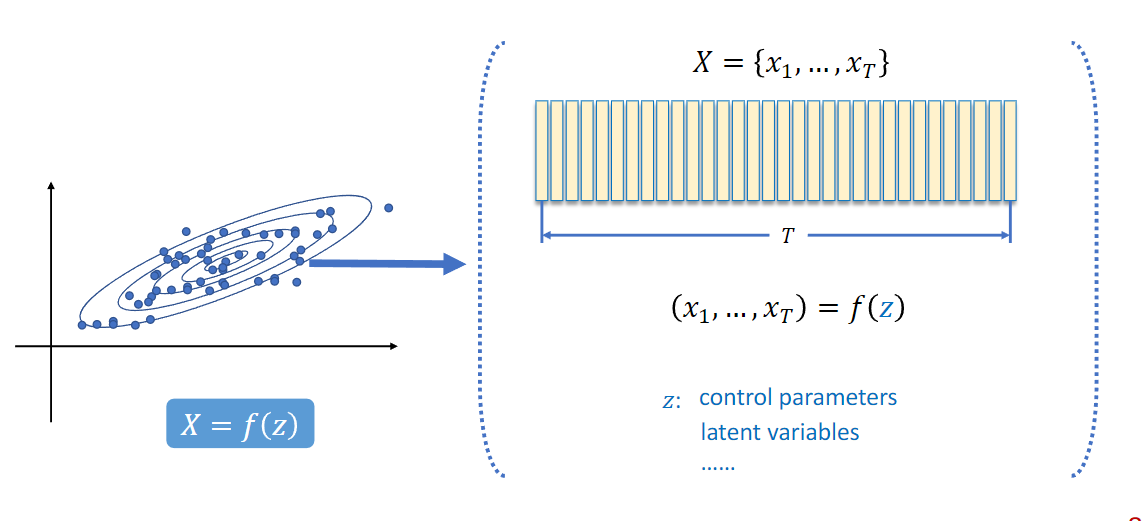
\includegraphics[width=\linewidth]{pic/1056/Learning Motion Models1}
    \end{subfigure}
    \begin{subfigure}{0.88\linewidth}
        \centering
        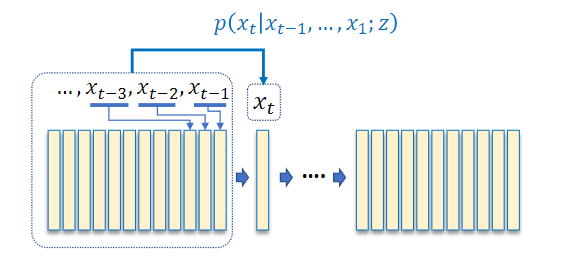
\includegraphics[width=\linewidth]{pic/1056/Learning Motion Models2}
    \end{subfigure}
    \caption{Two Perspectives on a Motion Sequence}
\end{figure}


\begin{enumerate}
    \item 给某个控制信号, 生成一个 motion $X=f(\bm z)$, $z$ 是控制信号的潜在表示. 
    \item 以之前的动作作为约束, 生成接下来的动作.
    \begin{align*}
        p(X|z)&=p(x_1,\dots,x_T|z)\\
        &=p(x_1)\prod_tp(x_t|x_{t-1},\dots,x_1;z)\\
        x_t &= f(x_{t-1},\dots,x_1;z)
    \end{align*}
    如果假设动作是马尔科夫过程, 则有 $x_t=f(x_{t-1};z)$
\end{enumerate}

\subsubsection{Autoregressive models}
考虑 马尔科夫 性质
\begin{align*}
    x_t = f(x_{t-1}; z)
\end{align*}
$z$ 表示控制信号的潜在表示.

先忽略 $z$
\begin{align*}
    x_t = f(x_{t-1})
\end{align*}
即给出一系列转移, 求分布. $\{ (x_{t-1}, x_t) \}\sim p(\bm X)$.

\begin{figure}[!htb]
    \centering
    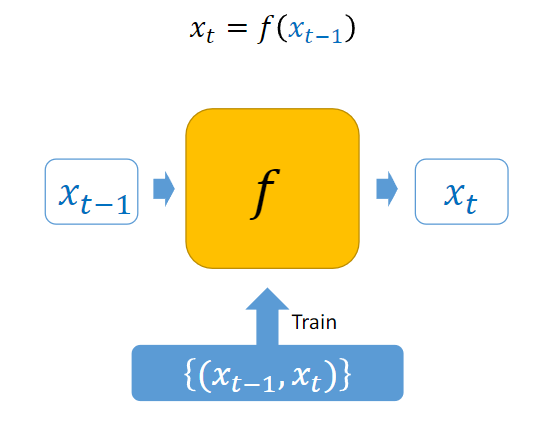
\includegraphics[width=0.309\linewidth]{pic/1056/Learning Motion Models3.png}
    \caption{Learning Motion Models}
\end{figure}

\begin{itemize}
    \item Interpolation: 使用对高维的插值处理,  其实插值的本质也可以看做拟合. 
    \item Neural Networks: 使用神经网络做拟合
\end{itemize}

\paragraph{Ambiguity Issue}
以 $x_t = f(x_{t-1})$ 为例, 对于一个输入, 可能对应多个输出. 这表示数据缺少约束. 学到的结果可能是个平均的动作. 

这表明 $x_t = f(x_{t-1})$ 不是一个单射, 需要加上额外的变量 $z$, 让其变为单射. i.e.
\begin{align*}
    x_t = f(x_{t-1};z)
\end{align*}

\begin{figure}[!htb]
    \centering
    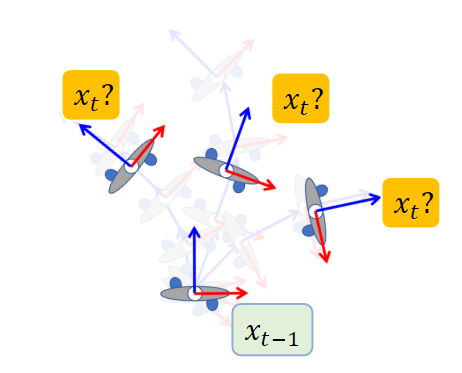
\includegraphics[width=0.309\linewidth]{pic/1056/Ambiguity Issue}
    \caption{Ambiguity Issue}
\end{figure}

\paragraph{PFNN: Phase-Functioned Neural Networks} 开创性工作, 表示神经网络可以用来做动作. 

用到了相位参数 (phase parameter), 将步幅的相位作为一个参数输入. 

但效果不好, 于是提出了 Mixture of Experts, 混合多个神经网络. 让一个专家学一个对应的相位的姿态, 然后根据权重混合专家的结果.

新的工作就是去学习权重混合, 而不是之前直接给定. 


\subsubsection{Generative models}
\begin{figure}[!htb]
    \centering
    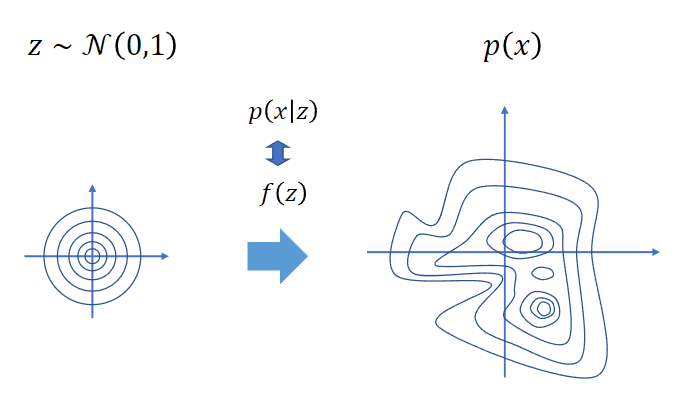
\includegraphics[width=0.42\linewidth]{pic/1056/Generative Models}
    \caption{Generative Models}
\end{figure}
从简单的概率分布( e.g. 正太分布)采样, 然后将其映射到目标概率空间. 



\begin{figure}[!htb]
    \centering
    \begin{subfigure}{0.88\linewidth}
        \centering
        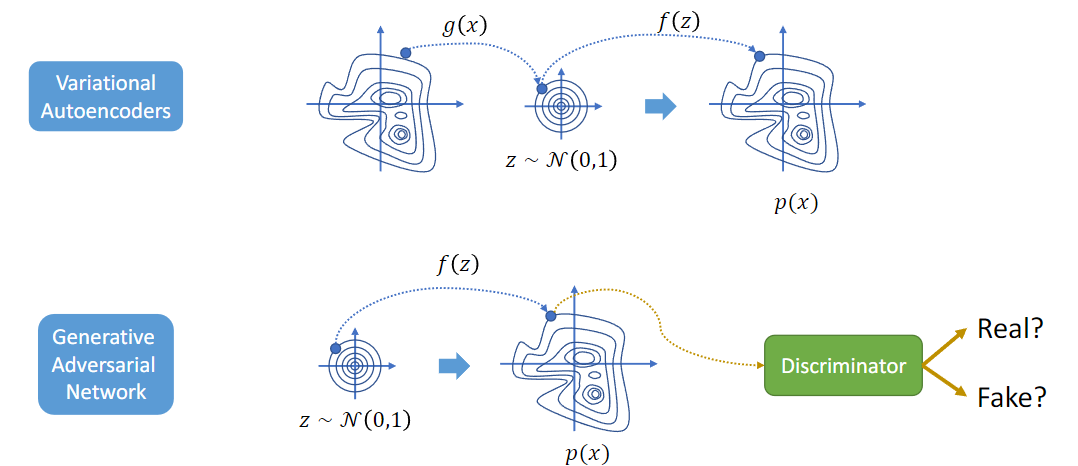
\includegraphics[width=\linewidth]{pic/1056/VAE and GAN}
        % \caption{}
    \end{subfigure}
    \begin{subfigure}{0.88\linewidth}
        \centering
        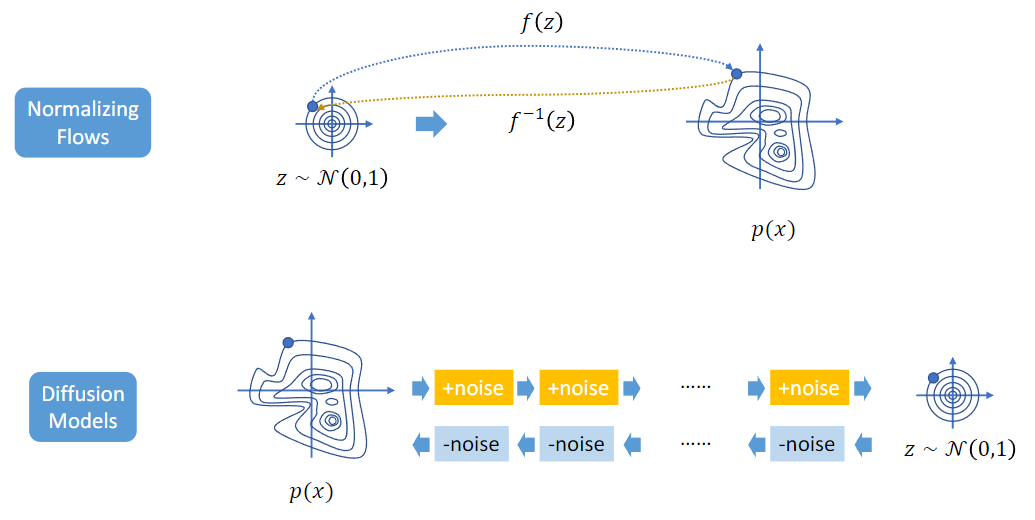
\includegraphics[width=\linewidth]{pic/1056/Normalizing Flows and Diffusion Models}
        % \caption{}
    \end{subfigure}
    \caption{流行的方法}
\end{figure}

目前流行的方法:
\begin{itemize}
    \item VAE (Variational Autoencoders)
    \item GAN(Generative Adversarial Network) 效果不好, 因为杀鸡用牛刀了. 加上物理控制就还行
    \item Normalizing Flows (要求函数可逆)
    \item Diffusion Models
\end{itemize}